\documentclass[spanish,letterpaper,oneside]{article}

% Datos del documento
\def\documenttitle {Suma y resta con fracciones}
\def\documentsubtitle {Temas selectos de matemáticas I}
\def\documentsubject {Actividad 2 · Ficha de trabajo resuelta}
\def\documentauthor {Mtro. Martín Jonathan de la Cruz Muñoz}
\def\coursename {Temas selectos de matemáticas I}
\def\coursecode {PFM02}

% Identidad institucional
\def\universityname {Instituto de Investigación, Innovación y Estudios de Posgrado para la Educación del Estado de Nuevo León}
\def\universityfaculty {Maestría en Aprendizaje y Enseñanza de las Matemáticas}
\def\universitydepartment {Temas selectos de matemáticas I}
\def\universitydepartmentimage {img/iiiepe/marca-iiiepe.png}
\def\universitydepartmentimagecfg {height=1.75cm}
\def\universitylocation {Monterrey, Nuevo León}
\def\studentfullname {Mtro. Martín Jonathan de la Cruz Muñoz}
\def\studentid {00874}
\def\studentemail {martin.delacruz@campus.iiiepe.edu.mx}
\def\programperiod {1er tetramestre, marzo--julio de 2026}
\def\programmodality {Modalidad presencial}
\def\programshort {MAEM}

\def\authortable {
  \begin{tabular}{ll}
    \textbf{Alumno:} & \studentfullname \\
    Matrícula: & \studentid \\
    Correo institucional: & \studentemail \\
    Unidad: & \coursename \\
    Programa: & \programshort \\
    Periodo: & \programperiod \\
    & \\
    \multicolumn{2}{l}{Fecha de realización: 13 de octubre de 2026} \\
    \multicolumn{2}{l}{\universitylocation}
  \end{tabular}
}

\input{template}

\usepackage{helvet}
\renewcommand{\familydefault}{\sfdefault}
\usepackage{array}
\usepackage{longtable}
\usepackage{pdflscape}
\usepackage{tikz}
\usepackage[most]{tcolorbox}
\usetikzlibrary{arrows.meta,positioning,calc,fit,backgrounds}

\definecolor{iiiepeNavy}{HTML}{163B5C}
\definecolor{iiiepeBlue}{HTML}{1F6F9F}
\definecolor{iiiepeAqua}{HTML}{20B7A8}
\definecolor{iiiepeOrange}{HTML}{F28C28}
\definecolor{iiiepePaper}{HTML}{F6F8F7}
\definecolor{iiiepeInk}{HTML}{1E2A32}
\def\portraittitlecolor {iiiepeNavy}
\setcitestyle{authoryear,open={(},close={)}}

\newcommand{\insertcoverwatermark}{%
  \AddToShipoutPictureBG*{%
    \begin{tikzpicture}[remember picture,overlay]
      \node[opacity=.09,inner sep=0pt] at (current page.center)
      {\includegraphics[width=.58\paperwidth]{img/iiiepe/logo-puntos.png}};
    \end{tikzpicture}%
  }%
}

\newtcolorbox{reportelecturabox}[1][]{%
  enhanced,breakable,
  colback=iiiepePaper,colframe=iiiepeNavy,
  boxrule=1pt,leftrule=4pt,arc=2pt,
  left=8pt,right=8pt,top=6pt,bottom=6pt,
  before skip=6pt,after skip=10pt,
  fonttitle=\bfseries\color{white},coltitle=white,
  colbacktitle=iiiepeNavy,
  attach boxed title to top left={xshift=8pt,yshift=-2pt},
  boxed title style={colback=iiiepeNavy,colframe=iiiepeNavy,arc=1pt},
  title={Reporte de lectura},#1}

\newtcolorbox{fichalecturabox}[1][]{%
  enhanced,breakable,
  colback=iiiepeAqua!7,colframe=iiiepeAqua!70!iiiepeNavy,
  boxrule=.6pt,arc=1pt,
  left=7pt,right=7pt,top=4pt,bottom=4pt,
  fontupper=\small,before upper={\setstretch{1.0}},
  fonttitle=\bfseries\color{iiiepeNavy},coltitle=iiiepeNavy,
  colbacktitle=iiiepeAqua!7,
  title={Ficha de la lectura},#1}



\usepackage{tabularx,colortbl,pgfplots,enumitem,needspace}\pgfplotsset{compat=1.18}\definecolor{iiiepePale}{HTML}{EEF5F8}
\setlength{\parskip}{5pt}\setlength{\parindent}{0pt}
\begin{document}\insertcoverwatermark\templatePortrait\templatePagecfg\templateFinalcfg\fancyfoot{}\fancyfoot[L]{\scriptsize IIIEPE · MAEM}\fancyfoot[C]{\scriptsize\thepage}\fancyfoot[R]{\scriptsize Actividad 2}\setstretch{1.3}\raggedbottom
\section{Sumar y restar cantidades comparables}
El denominador expresa la unidad fraccionaria. Por eso $1/2+1/3$ no es $2/5$: primero se construyen unidades equivalentes. Con sextos, $1/2=3/6$ y $1/3=2/6$, de modo que la suma es $5/6$. La equivalencia es el fundamento del algoritmo y permite decidir si un resultado tiene sentido.

\begin{center}
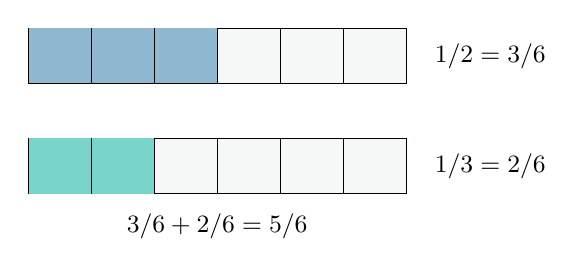
\begin{tikzpicture}[x=.8cm,y=.7cm,font=\small]
\foreach \y/\v in {2/1,0/2}{\foreach \i in {0,...,5}{\draw[fill=iiiepePaper] (\i,\y) rectangle +(1,1);}}
\fill[iiiepeBlue!50] (0,2) rectangle (3,3);\fill[iiiepeAqua!60] (0,0) rectangle (2,1);
\foreach \i in {0,...,6}{\draw (\i,2)--(\i,3);\draw (\i,0)--(\i,1);}
\node[right] at (6.3,2.5){$1/2=3/6$};\node[right] at (6.3,.5){$1/3=2/6$};\node at (3,-.6){$3/6+2/6=5/6$};\end{tikzpicture}
\end{center}
\section{Ejercicios de la ficha oficial}
\subsection*{Conversión de fracciones impropias y mixtas} Para $a/b$, se divide $a=qb+r$, con $0\le r<b$; entonces $a/b=q+r/b$. Para $n+a/b$, se calcula $(nb+a)/b$. Los incisos se presentan en las tablas siguientes.\subsection*{Simplificación}


{\small\setstretch{1.1}\renewcommand{\arraystretch}{1.25}
\begin{longtable}{|>{\raggedright\arraybackslash}p{\dimexpr0.5\linewidth-2\tabcolsep-2\arrayrulewidth\relax}|>{\raggedright\arraybackslash}p{\dimexpr0.5\linewidth-2\tabcolsep-2\arrayrulewidth\relax}|}\hline
\rowcolor{iiiepePale} \textbf{Expresión} & \textbf{Procedimiento y resultado} \\\hline
\endfirsthead
\hline
\rowcolor{iiiepePale} \textbf{Expresión} & \textbf{Procedimiento y resultado} \\\hline
\endhead
$\frac{4}{20}$ & $\frac{1}{5}$ \\\hline
$\frac{6}{24}$ & $\frac{1}{4}$ \\\hline
$\frac{12}{30}$ & $\frac{2}{5}$ \\\hline
$\frac{9}{27}$ & $\frac{1}{3}$ \\\hline
$\frac{24}{32}$ & $\frac{3}{4}$ \\\hline
$\frac{15}{25}$ & $\frac{3}{5}$ \\\hline
\end{longtable}}

\subsection*{Impropias a mixtas}


{\small\setstretch{1.1}\renewcommand{\arraystretch}{1.25}
\begin{longtable}{|>{\raggedright\arraybackslash}p{\dimexpr0.5\linewidth-2\tabcolsep-2\arrayrulewidth\relax}|>{\raggedright\arraybackslash}p{\dimexpr0.5\linewidth-2\tabcolsep-2\arrayrulewidth\relax}|}\hline
\rowcolor{iiiepePale} \textbf{Expresión} & \textbf{Procedimiento y resultado} \\\hline
\endfirsthead
\hline
\rowcolor{iiiepePale} \textbf{Expresión} & \textbf{Procedimiento y resultado} \\\hline
\endhead
$\frac{5}{4}$ & $1\frac{1}{4}$ \\\hline
$\frac{8}{3}$ & $2\frac{2}{3}$ \\\hline
$\frac{7}{4}$ & $1\frac{3}{4}$ \\\hline
$\frac{50}{3}$ & $16\frac{2}{3}$ \\\hline
$\frac{11}{2}$ & $5\frac{1}{2}$ \\\hline
$\frac{4}{3}$ & $1\frac{1}{3}$ \\\hline
\end{longtable}}

\subsection*{Mixtas a impropias}


{\small\setstretch{1.1}\renewcommand{\arraystretch}{1.25}
\begin{longtable}{|>{\raggedright\arraybackslash}p{\dimexpr0.5\linewidth-2\tabcolsep-2\arrayrulewidth\relax}|>{\raggedright\arraybackslash}p{\dimexpr0.5\linewidth-2\tabcolsep-2\arrayrulewidth\relax}|}\hline
\rowcolor{iiiepePale} \textbf{Expresión} & \textbf{Procedimiento y resultado} \\\hline
\endfirsthead
\hline
\rowcolor{iiiepePale} \textbf{Expresión} & \textbf{Procedimiento y resultado} \\\hline
\endhead
$5+\frac{3}{2}$ & $\frac{5(2)+3}{2}=\frac{13}{2}$ \\\hline
$9+\frac{2}{3}$ & $\frac{9(3)+2}{3}=\frac{29}{3}$ \\\hline
$8+\frac{3}{4}$ & $\frac{8(4)+3}{4}=\frac{35}{4}$ \\\hline
$15+\frac{1}{3}$ & $\frac{15(3)+1}{3}=\frac{46}{3}$ \\\hline
$7+\frac{7}{8}$ & $\frac{7(8)+7}{8}=\frac{63}{8}$ \\\hline
$2+\frac{3}{16}$ & $\frac{2(16)+3}{16}=\frac{35}{16}$ \\\hline
\end{longtable}}

\subsection*{Mismo denominador}


{\small\setstretch{1.1}\renewcommand{\arraystretch}{1.25}
\begin{longtable}{|>{\raggedright\arraybackslash}p{\dimexpr0.5\linewidth-2\tabcolsep-2\arrayrulewidth\relax}|>{\raggedright\arraybackslash}p{\dimexpr0.5\linewidth-2\tabcolsep-2\arrayrulewidth\relax}|}\hline
\rowcolor{iiiepePale} \textbf{Expresión} & \textbf{Procedimiento y resultado} \\\hline
\endfirsthead
\hline
\rowcolor{iiiepePale} \textbf{Expresión} & \textbf{Procedimiento y resultado} \\\hline
\endhead
$\frac72+\frac52$ & $\frac{7+5}2=6$ \\\hline
$\frac87+\frac17+\frac27$ & $\frac{11}7=1\frac47$ \\\hline
$\frac{17}4-\frac{10}4$ & $\frac74=1\frac34$ \\\hline
$\frac{12}9-\frac39-\frac49$ & $\frac59$ \\\hline
\end{longtable}}

\subsection*{Producto cruzado}


{\small\setstretch{1.1}\renewcommand{\arraystretch}{1.25}
\begin{longtable}{|>{\raggedright\arraybackslash}p{\dimexpr0.5\linewidth-2\tabcolsep-2\arrayrulewidth\relax}|>{\raggedright\arraybackslash}p{\dimexpr0.5\linewidth-2\tabcolsep-2\arrayrulewidth\relax}|}\hline
\rowcolor{iiiepePale} \textbf{Expresión} & \textbf{Procedimiento y resultado} \\\hline
\endfirsthead
\hline
\rowcolor{iiiepePale} \textbf{Expresión} & \textbf{Procedimiento y resultado} \\\hline
\endhead
$\frac12+\frac37$ & $\frac{1(7)+3(2)}{14}=\frac{13}{14}$ \\\hline
$\frac69+\frac2{10}$ & $\frac{60+18}{90}=\frac{13}{15}$ \\\hline
$\frac32-\frac35$ & $\frac{15-6}{10}=\frac9{10}$ \\\hline
$\frac{10}3-\frac94$ & $\frac{40-27}{12}=\frac{13}{12}$ \\\hline
\end{longtable}}

\subsection*{Fracciones equivalentes}


{\small\setstretch{1.1}\renewcommand{\arraystretch}{1.25}
\begin{longtable}{|>{\raggedright\arraybackslash}p{\dimexpr0.5\linewidth-2\tabcolsep-2\arrayrulewidth\relax}|>{\raggedright\arraybackslash}p{\dimexpr0.5\linewidth-2\tabcolsep-2\arrayrulewidth\relax}|}\hline
\rowcolor{iiiepePale} \textbf{Expresión} & \textbf{Procedimiento y resultado} \\\hline
\endfirsthead
\hline
\rowcolor{iiiepePale} \textbf{Expresión} & \textbf{Procedimiento y resultado} \\\hline
\endhead
$\frac34+\frac12$ & $\frac34+\frac24=\frac54$ \\\hline
$\frac74+\frac3{20}$ & $\frac{35}{20}+\frac3{20}=\frac{19}{10}$ \\\hline
$\frac23+\frac17$ & $\frac{14}{21}+\frac3{21}=\frac{17}{21}$ \\\hline
$\frac49-\frac13$ & $\frac49-\frac39=\frac19$ \\\hline
$\frac7{15}-\frac25$ & $\frac7{15}-\frac6{15}=\frac1{15}$ \\\hline
$\frac53-\frac4{27}$ & $\frac{45}{27}-\frac4{27}=\frac{41}{27}$ \\\hline
\end{longtable}}

\section{Situaciones contextualizadas}

{\small\setstretch{1.1}\renewcommand{\arraystretch}{1.25}
\begin{longtable}{|>{\raggedright\arraybackslash}p{\dimexpr0.22\linewidth-2\tabcolsep-2\arrayrulewidth\relax}|>{\raggedright\arraybackslash}p{\dimexpr0.78\linewidth-2\tabcolsep-2\arrayrulewidth\relax}|}\hline
\rowcolor{iiiepePale} \textbf{Caso} & \textbf{Procedimiento e interpretación} \\\hline
\endfirsthead
\hline
\rowcolor{iiiepePale} \textbf{Caso} & \textbf{Procedimiento e interpretación} \\\hline
\endhead
1 & La receta para 4 porciones usa $1\frac12$ tazas de agua y $1/4$ de piloncillo. Para 12 porciones, el factor es $12/4=3$: agua $3(3/2)=9/2=4\frac12$ tazas; piloncillo $3(1/4)=3/4$ de taza. \\\hline
2 & Pizza: $1/3+1/4=(4+3)/12=7/12$ consumidos. \\\hline
3 & Caramelos: $1-(1/4+1/2)=1/4$ de bolsa restante. \\\hline
4 & Distancia: $2/8+5\frac23=1/4+17/3=71/12=5\frac{11}{12}$ km. \\\hline
5 & Yeso: $1\frac12-6/4=3/2-3/2=0$ kg. \\\hline
6 & Trigo: $1-(1/8+1/4)=5/8$ del rancho. \\\hline
\end{longtable}}



{\small\setstretch{1.1}\renewcommand{\arraystretch}{1.25}
\begin{longtable}{|>{\raggedright\arraybackslash}p{\dimexpr0.22\linewidth-2\tabcolsep-2\arrayrulewidth\relax}|>{\raggedright\arraybackslash}p{\dimexpr0.78\linewidth-2\tabcolsep-2\arrayrulewidth\relax}|}\hline
\rowcolor{iiiepePale} \textbf{Caso} & \textbf{Procedimiento e interpretación} \\\hline
\endfirsthead
\hline
\rowcolor{iiiepePale} \textbf{Caso} & \textbf{Procedimiento e interpretación} \\\hline
\endhead
7 & Con las proporciones de la tabla: $1-(1/4+1/6+1/3)=1-9/12=1/4$ sin deporte favorito. \\\hline
8 & Antonio: $4\frac12+3\frac58+3\frac34=(36+29+30)/8=95/8=11\frac78$ km. \\\hline
9 & Espesores: $7/12+5/6+2/3=(7+10+8)/12=25/12=2\frac1{12}$ pulgadas. \\\hline
10 & Rectángulo: $P=2(4\frac34+2\frac12)=2(19/4+10/4)=29/2$ cm, opción a. \\\hline
\end{longtable}}

\section{Dos estrategias y una comprobación}
Para $7/4+3/20$, el mínimo común múltiplo de 4 y 20 es 20. La equivalencia $7/4=35/20$ produce $(35+3)/20=38/20=19/10$. El producto cruzado también es válido: $(7\cdot20+3\cdot4)/80=152/80=19/10$, pero utiliza números mayores. Comparar las estrategias permite elegir con criterio sin convertir una en la única ruta legítima.
Para $4/9-1/3$, se representa $1/3$ como $3/9$ y se resta $(4-3)/9=1/9$. La comprobación $1/9+1/3=4/9$ utiliza la operación inversa. El error $4/9-1/3=3/6$ mezcla unidades distintas y puede refutarse además por estimación: $4/9$ es menor que $1/2$, de modo que al restar una cantidad positiva no puede obtenerse $1/2$.
El inciso $5\frac32$ del recurso tiene una parte fraccionaria impropia: se interpreta como $5+3/2=13/2=6\frac12$. La forma convencional exige una parte fraccionaria menor que la unidad. Señalar esta particularidad evita aprender una notación ambigua como norma.
\section{Secuencia de aplicación y evaluación}
Justificar suma y resta con unidades fraccionarias comparables. La duración propuesta es de 60 minutos, ajustable al diagnóstico y a los recursos. Esta planeación sigue la progresión de los recursos institucionales (IIIEPE, 2026); los tiempos y apoyos son decisiones de codiseño, no datos de una aplicación ya realizada.

{\small\setstretch{1.1}\renewcommand{\arraystretch}{1.25}
\begin{longtable}{|>{\raggedright\arraybackslash}p{\dimexpr0.23\linewidth-2\tabcolsep-2\arrayrulewidth\relax}|>{\raggedright\arraybackslash}p{\dimexpr0.49\linewidth-2\tabcolsep-2\arrayrulewidth\relax}|>{\raggedright\arraybackslash}p{\dimexpr0.28\linewidth-2\tabcolsep-2\arrayrulewidth\relax}|}\hline
\rowcolor{iiiepePale} \textbf{Fase y tiempo} & \textbf{Actividad y mediación} & \textbf{Evidencia} \\\hline
\endfirsthead
\hline
\rowcolor{iiiepePale} \textbf{Fase y tiempo} & \textbf{Actividad y mediación} & \textbf{Evidencia} \\\hline
\endhead
1. Antecedentes (8 min) & Representar dos porciones de igual unidad y anticipar una suma. & Predicción individual y pregunta. \\\hline
2. Explicación (12 min) & Construir equivalencias con sextos y comparar dos algoritmos. & Plan explicado y criterios. \\\hline
3. Práctica (20 min) & Resolver suma, resta y un problema de complemento. & Registro o procedimiento trazable. \\\hline
4. Evaluación (12 min) & Explicar el denominador y verificar una respuesta con operación inversa. & Argumento con comprobación. \\\hline
5. Retroalimentación (8 min) & Revisar un error de suma de denominadores y resolver otro caso. & Versión revisada y justificación. \\\hline
\end{longtable}}
\subsection{Criterios observables y retroalimentación}

{\small\setstretch{1.1}\renewcommand{\arraystretch}{1.25}
\begin{longtable}{|>{\raggedright\arraybackslash}p{\dimexpr0.22\linewidth-2\tabcolsep-2\arrayrulewidth\relax}|>{\raggedright\arraybackslash}p{\dimexpr0.4\linewidth-2\tabcolsep-2\arrayrulewidth\relax}|>{\raggedright\arraybackslash}p{\dimexpr0.38\linewidth-2\tabcolsep-2\arrayrulewidth\relax}|}\hline
\rowcolor{iiiepePale} \textbf{Criterio} & \textbf{Evidencia de logro} & \textbf{Acción si necesita apoyo} \\\hline
\endfirsthead
\hline
\rowcolor{iiiepePale} \textbf{Criterio} & \textbf{Evidencia de logro} & \textbf{Acción si necesita apoyo} \\\hline
\endhead
Unidad fraccionaria & Explica unidad fraccionaria con un caso de la actividad. & Pedir una representación concreta y contrastar dos casos. \\\hline
Equivalencias y algoritmo & Conserva equivalencias y algoritmo en el desarrollo y justifica sus pasos. & Modelar un paso, retirar gradualmente la ayuda y solicitar otro caso. \\\hline
Problema contextual & Utiliza problema contextual para contrastar una respuesta o representación. & Comparar la evidencia inicial y la corregida con una pregunta específica. \\\hline
Comprobación e interpretación & Relaciona comprobación e interpretación con la conclusión y un límite del problema. & Solicitar una comprobación independiente y un caso de transferencia. \\\hline
\end{longtable}}
El instrumento es una propuesta docente. Cada criterio se registra como logrado con autonomía, logrado con apoyo o aún no demostrado; no se asigna una calificación observada sin aplicar la actividad. En la coevaluación, un compañero verifica un criterio y formula una pregunta; en la autoevaluación, el estudiante explica una corrección; el docente contrasta ambas evidencias y decide el siguiente apoyo.\subsection{Participación y apoyos}
La inclusión se concreta en alternativas de representación y de acceso; el pensamiento crítico, en justificar y contrastar. Los roles de cálculo, registro y explicación se rotan para que todos produzcan una evidencia individual. Quien necesita apoyo dispone de un ejemplo parcial y preguntas graduadas; quien ya domina el procedimiento analiza un contraejemplo o cambia una condición. Estas acciones deben observarse durante la aplicación para valorar su funcionamiento.

\section{Diseño didáctico y reflexión}
Iniciaría con una receta o el apilamiento de materiales del taller. Representaría primero las partes con tiras de igual longitud para que cada denominador conserve su significado. El desarrollo avanzaría desde denominadores iguales hacia equivalencias y problemas de complemento. En el cierre, cada estudiante justificaría una respuesta y contrastaría su procedimiento con otro.
En mi acercamiento a una enseñanza humanista, la precisión no exige que todos avancen al mismo ritmo. Quien suma denominadores necesita reconstruir la unidad; quien ya resuelve puede comparar la eficiencia del mínimo común múltiplo con el producto de denominadores. La retroalimentación debe indicar qué cambiar y permitir una nueva resolución, sin reducir la valoración a rapidez o calificación.

\needspace{5\baselineskip}\section*{Referencias}
{\setstretch{1.15}\setlength{\parskip}{6pt}
\par\hangindent=1.27cm\hangafter=1  IIIEPE. (2026). \textit{Sesión 02: Suma y resta con fracciones}. Ficha de Temas selectos de matemáticas I, EVA posgrado.
\par\hangindent=1.27cm\hangafter=1  Secretaría de Educación Pública. (2024). \textit{Programa de estudio para la educación secundaria: Programa sintético de la Fase 6}. SEP.
}

\end{document}
